%-------------------------------------------------------------------- Comente: Stackelberg
\needspace{8\baselineskip}
\tema{Comente: Stackelberg vs Cournot}
\question \textbf{Comente.} Considere 2 empresas. Si comparamos con los resultados obtenidos en una competencia simultánea à la Cournot, tendremos que tanto los consumidores como la firma líder estarán mejor bajo una competencia secuencial tipo Stackelberg.
\needspace{5\baselineskip}
\begin{solution}
Verdadero. Ante un juego secuencial tipo Stackelberg, la firma líder expandirá su producción respecto al juego simultáneo debido a que sabe que la firma seguidora ajustará su producción a la baja para no deprimir demasiado el precio. Lo anterior se traduce en mayores niveles de producción en el agregado, menores precios y, por lo tanto, mayores beneficios para los consumidores y para la firma líder (respecto al juego simultáneo).

\end{solution}

%-------------------------------------------------------------------- Stackelberg numérico
\needspace{8\baselineskip}
\tema{Cournot y Stackelberg con costos asimétricos}
\question La curva de demanda inversa de un bien está dada por $P(Q) = 240 - 2Q$. Existen dos firmas con funciones de costos $CT_1(q_1) = 40q_1$ y $CT_2(q_2) = 80q_2$.
\begin{parts}
\part Si ambas firmas compiten à la Cournot, determine las funciones de reacción de ambas. ¿Cuál es el nivel de producción y el precio de equilibrio en este caso? ¿Cuáles son los beneficios de ambas empresas?
\needspace{5\baselineskip}
\begin{solution}
Cada firma maximiza sus utilidades:
\begin{gather*}
  \max_{q_1}\ \pi_1 = (240 - 2Q - 40)q_1 \;\Rightarrow\; \frac{\partial\pi_1}{\partial q_1} = 240 - 2q_2 - 4q_1 - 40 = 0 \\ \;\Rightarrow\; q_1(q_2) = \frac{200 - 2q_2}{4}, \\
  \max_{q_2}\ \pi_2 = (240 - 2Q - 80)q_2 \;\Rightarrow\; \frac{\partial\pi_2}{\partial q_2} = 240 - 2q_1 - 4q_2 - 80 = 0 \\ \;\Rightarrow\; q_2(q_1) = \frac{160 - 2q_1}{4}.
\end{gather*}
Reemplazando una en la otra se obtiene
\[
  q_1^* = 40, \qquad q_2^* = 20, \qquad P^* = 240 - 2\cdot 60 = 120, \qquad \pi_1^* = 3200, \qquad \pi_2^* = 800 .
\]

\end{solution}

\part Suponga que las dos empresas de la industria se comportan à la Stackelberg (en cantidad), de modo que la empresa 1 actúa como líder y la 2 como seguidora. ¿Cuál sería la producción y el precio de equilibrio de mercado? ¿Cuánto producirá la empresa 1? ¿Cuánto producirá la empresa 2? ¿Cuáles serán los beneficios de ambas empresas?
\needspace{5\baselineskip}
\begin{solution}
Es un juego secuencial en dos etapas, que se resuelve por inducción hacia atrás. En $t=2$ la seguidora maximiza
\[
\begin{gathered}
  \max_{q_2}\ \pi_2 = (240 - 2(q_1+q_2))q_2 - 80q_2 \\
  \;\Rightarrow\; 240 - 2q_1 - 4q_2 - 80 = 0 \\
  \;\Rightarrow\; q_2(q_1) = \frac{160 - 2q_1}{4}.
\end{gathered}
\]
La firma 1 conoce la estrategia de la firma 2, por lo que escoge su cantidad óptima usando esta información (reemplaza la restricción $q_2 = q_2(q_1)$):
\[
  \max_{q_1}\ \pi_1 = \Bigl(240 - 2\bigl(q_1 + \tfrac{160 - 2q_1}{4}\bigr)\Bigr)q_1 - 40q_1
  \;\Rightarrow\; 160 - 2q_1 - 40 = 0 \;\Rightarrow\; q_1^* = 60 .
\]
La mejor respuesta de la firma 2 es producir $q_2^* = \frac{160-120}{4} = 10$. La producción total es $Q^* = 70$ y el precio $P^* = 240 - 140 = 100$. Las utilidades son
\[
  \pi_1^* = (100-40)\cdot 60 = 3600, \qquad \pi_2^* = (100-80)\cdot 10 = 200 .
\]
Comparando con Cournot, la líder produce y gana más, la seguidora produce y gana menos, y el precio es menor.

\end{solution}
\end{parts}

%-------------------------------------------------------------------- Comente: timing
\needspace{8\baselineskip}
\tema{Comente: timing de las decisiones en cantidades}
\question \textbf{Comente.} En una competencia de cantidades, y asumiendo simetría en la estructura de costos, da lo mismo si las firmas deciden el tamaño de producción en el mismo período o en períodos distintos, pues se llega al mismo equilibrio.
\needspace{5\baselineskip}
\begin{solution}
Falso. El \emph{timing} de la toma de decisiones de las firmas sí influye en el resultado final de equilibrio. Cuando las firmas deciden sus producciones de forma simultánea, nos encontramos en el típico caso de competencia à la Cournot, donde la producción y los beneficios son iguales entre ambas firmas. Cuando una firma decide su producción antes que otra, esto corresponde a un modelo Stackelberg, donde la firma que decide primero su producción tendrá una mayor participación de mercado y mayores beneficios.

\end{solution}

%-------------------------------------------------------------------- Comente: credibilidad
\needspace{8\baselineskip}
\tema{Comente: credibilidad en Stackelberg}
\question \textbf{Comente.} El elemento clave en el modelo de Stackelberg es la credibilidad. En concreto, si no es creíble que alguna firma pueda ajustar su plan de producción, entonces los resultados de este juego secuencial serán los mismos que los del juego simultáneo.
\needspace{5\baselineskip}
\begin{solution}
Falso. La credibilidad juega un rol clave en el modelo secuencial al interpretar el papel de una amenaza creíble. Para que una firma sea líder, necesitamos que, por ejemplo, no pueda ajustar su producción, es decir, que el compromiso de no ajustar su producción sea creíble. Si la firma seguidora sabe que tal compromiso es creíble (o, equivalentemente, que no es creíble que la firma líder pueda ajustar su producción), entonces efectivamente tendremos un juego secuencial, cuyos resultados serán diferentes al juego simultáneo.

\end{solution}

%-------------------------------------------------------------------- Comente: líder produce menos
\needspace{8\baselineskip}
\tema{Comente: cantidad del líder en Stackelberg}
\question \textbf{Comente.} En la competencia à la Stackelberg, el \emph{timing} indica que la firma que mueve primero producirá una cantidad menor para cobrar un precio alto del bien que produce y, por ende, maximizar sus beneficios.
\needspace{5\baselineskip}
\begin{solution}
Falso. La firma que mueve primero escogerá una cantidad \emph{mayor}. Luego, la firma seguidora escogerá una cantidad menor para no deprimir el precio y obtener beneficios positivos.

\end{solution}

%-------------------------------------------------------------------- Comente: Cournot vs Stackelberg beneficios
\needspace{8\baselineskip}
\tema{Comente: producción y beneficios del líder y seguidor}
\question \textbf{Comente.} En competencia à la Cournot con dos firmas, la cantidad producida por la firma que escoge primero en el modelo de Stackelberg es mayor que en el modelo de decisiones simultáneas, y los beneficios de las firmas también son mayores.
\needspace{5\baselineskip}
\begin{solution}
La primera afirmación es verdadera, ya que la firma líder sí producirá más que en el caso de decisiones simultáneas. Sin embargo, la segunda parte del comente es falsa, ya que solo aumentarán los beneficios de la firma que escoge primero, mientras que en el caso de la firma seguidora sus beneficios serán menores que si las decisiones fuesen simultáneas.

\end{solution}

%-------------------------------------------------------------------- Comente: ventaja primer movimiento
\needspace{8\baselineskip}
\tema{Comente: ventaja de mover primero}
\question \textbf{Comente.} En Stackelberg, siempre será ventajoso mover primero.
\needspace{5\baselineskip}
\begin{solution}
Falso. Cuando la competencia es en precios, resulta ventajoso mover después, dado que puedo reducir el precio ofrecido por la primera firma y quedarme con una mayor demanda.

\end{solution}

%-------------------------------------------------------------------- Stackelberg precios distintos
\needspace{8\baselineskip}
\tema{Stackelberg con funciones de precio distintas}
\question En una economía solo existen dos firmas que abastecen todo el mercado. Sus funciones de precio son
\begin{align*}
  P_A &= 80 - \tfrac{3}{2}q_A - q_B \\
  P_B &= 80 - \tfrac{3}{2}q_B - q_A
\end{align*}
Asuma que ninguna posee costos de producción y que la firma $A$ es líder y $B$ seguidora.
\begin{parts}
\part Suponga que las dos empresas de la industria se comportan à la Stackelberg (en cantidad). ¿Cuál sería la producción y el precio de equilibrio de mercado? ¿Cuánto producirá la empresa $A$? ¿Cuánto producirá la empresa $B$? ¿Cuáles serán los beneficios de ambas empresas?
\needspace{5\baselineskip}
\begin{solution}
Es un juego secuencial en dos etapas, que se resuelve por inducción hacia atrás. En $t=2$ la seguidora maximiza
\[
  \max_{q_B}\ \pi_B = \bigl(80 - \tfrac{3}{2}q_B - q_A\bigr)q_B
  \;\Rightarrow\; 80 - 3q_B - q_A = 0
  \;\Rightarrow\; q_B(q_A) = \frac{80}{3} - \frac{1}{3}q_A .
\]
La firma $A$ conoce la estrategia de la firma $B$, por lo que escoge su cantidad óptima usando esta información:
\[
  \max_{q_A}\ \pi_A = \bigl(80 - \tfrac{3}{2}q_A - q_B\bigr)q_A
  \quad \text{s.a.} \quad q_B = \frac{80}{3} - \frac{1}{3}q_A .
\]
Reemplazando la restricción,
\[
  \max_{q_A}\ \pi_A = \Bigl(80 - \tfrac{3}{2}q_A - \tfrac{80}{3} + \tfrac{1}{3}q_A\Bigr)q_A
  \;\Rightarrow\; \frac{160}{3} - \frac{7}{3}q_A = 0
  \;\Rightarrow\; q_A^* = \frac{160}{7} \approx 22{,}86 .
\]
Por lo tanto, la mejor respuesta de la firma $B$ es producir $q_B^* = \frac{400}{21} \approx 19{,}05$, y la producción total es $Q^* \approx 41{,}90$. Los precios (distintos, pues las funciones de precio lo son) y los beneficios son
\[
  P_A^* = \tfrac{80}{3} \approx 26{,}67, \quad P_B^* = \tfrac{200}{7} \approx 28{,}57, \qquad
  \pi_A^* \approx 609{,}5, \quad \pi_B^* \approx 544{,}2 .
\]

\end{solution}

\part \emph{(Propuesto)} Suponga ahora que las empresas enfrentan costos $C_{mg,A} = 2$ y $C_{mg,B} = 3$. Encuentre lo solicitado en (a) con la nueva información.
\needspace{5\baselineskip}
\begin{solution}
Se procede igual, con los nuevos costos. La seguidora resuelve $80 - 3q_B - q_A - 3 = 0$, es decir $q_B(q_A) = \frac{77}{3} - \frac{1}{3}q_A$. La líder maximiza
\[
  \max_{q_A}\ \pi_A = \Bigl(80 - \tfrac{3}{2}q_A - \tfrac{77}{3} + \tfrac{1}{3}q_A - 2\Bigr)q_A
  \;\Rightarrow\; \frac{157}{3} - \frac{7}{3}q_A = 0
  \;\Rightarrow\; q_A^* = \frac{157}{7} \approx 22{,}43 ,
\]
y $q_B^* = \frac{382}{21} \approx 18{,}19$. Los precios son $P_A^* \approx 28{,}17$ y $P_B^* \approx 30{,}29$, y los beneficios $\pi_A^* \approx 586{,}9$ y $\pi_B^* \approx 496{,}3$.

\end{solution}
\end{parts}

%-------------------------------------------------------------------- Comente: Stackelberg eficiente
\needspace{8\baselineskip}
\tema{Comente: eficiencia de Stackelberg vs Cournot}
\question \textbf{Comente.} ¿Cuándo la competencia tipo Stackelberg puede ser más eficiente que Cournot? ¿Cuándo podría ser más ineficiente que Cournot?
\needspace{5\baselineskip}
\begin{solution}
En caso de que tanto la firma líder como la seguidora sean igual de eficientes, el resultado Stackelberg será más eficiente que Cournot: el precio es menor y la cantidad producida es mayor.

En caso de que la líder sea más ineficiente, puede ocurrir que Stackelberg no sea más eficiente que Cournot, pues parte de la producción se traspasa a la firma más ineficiente (las firmas más ineficientes en Cournot producen menos).

\end{solution}

%-------------------------------------------------------------------- Comente: EN vs EPS
\needspace{8\baselineskip}
\tema{Comente: equilibrio de Nash y equilibrio perfecto en subjuegos}
\question \textbf{Comente.} Defina equilibrio de Nash y equilibrio perfecto en subjuegos. ¿Cómo se relacionan?
\needspace{5\baselineskip}
\begin{solution}
Un equilibrio de Nash (EN) es un resultado de un juego (conjunto de estrategias) tal que ningún individuo tiene incentivo a cambiar su estrategia. Un equilibrio perfecto en subjuegos (EPS) es un equilibrio de Nash creíble en un juego secuencial: es un EN en todos los subjuegos. Todo EPS es un EN, pero no todo EN es un EPS.

\end{solution}

%-------------------------------------------------------------------- Juego extensivo
\needspace{8\baselineskip}
\tema{Juego en forma extensiva: Nash y perfección en subjuegos}
\question Considere el siguiente juego secuencial. El jugador 1 elige entre $A$, $B$ y $C$. Si elige $C$, el juego termina con pagos $(2,2)$. Si elige $A$, el jugador 2 elige entre $a$ y $b$; si elige $b$ el juego termina con pagos $(1,-1)$, y si elige $a$ el jugador 1 elige entre $X$ (pagos $(3,0)$) e $Y$ (pagos $(0,3)$). Si elige $B$, el jugador 1 elige entre $\alpha$ y $\beta$; si elige $\beta$ el juego termina con pagos $(1,-1)$, y si elige $\alpha$ el jugador 2 elige entre $x$ (pagos $(3,0)$) e $y$ (pagos $(0,3)$). (Los pagos se escriben como $(\text{jugador 1},\text{jugador 2})$.)
\begin{center}
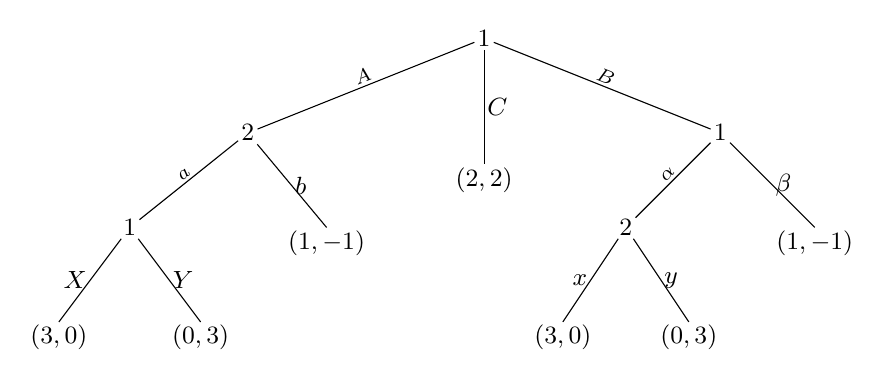
\begin{tikzpicture}[x=1cm,y=1cm,font=\small,every node/.style={inner sep=1pt},
  lev/.style={sloped,midway,above,font=\scriptsize}]
  \node (r) at (0,0) {1};
  \node (n2a) at (-3,-1.2) {2};
  \node (n1a) at (-4.5,-2.4) {1};
  \node (n1b) at (3,-1.2) {1};
  \node (n2b) at (1.8,-2.4) {2};
  \draw (r) -- (n2a) node[lev] {$A$};
  \draw (r) -- (0,-1.6) node[below,align=center] {$(2,2)$} node[midway,right] {$C$};
  \draw (r) -- (n1b) node[lev] {$B$};
  \draw (n2a) -- (n1a) node[lev] {$a$};
  \draw (n2a) -- (-2,-2.4) node[below,align=center] {$(1,-1)$} node[midway,right] {$b$};
  \draw (n1a) -- (-5.4,-3.6) node[below] {$(3,0)$} node[midway,left] {$X$};
  \draw (n1a) -- (-3.6,-3.6) node[below] {$(0,3)$} node[midway,right] {$Y$};
  \draw (n1b) -- (n2b) node[lev] {$\alpha$};
  \draw (n1b) -- (4.2,-2.4) node[below,align=center] {$(1,-1)$} node[midway,right] {$\beta$};
  \draw (n2b) -- (1,-3.6) node[below] {$(3,0)$} node[midway,left] {$x$};
  \draw (n2b) -- (2.6,-3.6) node[below] {$(0,3)$} node[midway,right] {$y$};
\end{tikzpicture}
\end{center}
\begin{parts}
\part Encuentre el equilibrio de Nash (perfecto en subjuegos).
\needspace{5\baselineskip}
\begin{solution}
Resolvemos por inducción hacia atrás, empezando desde abajo. En el nodo inferior izquierdo, el jugador 1 escoge $X$ (3 > 0). En el nodo inferior derecho, el jugador 2 escoge $y$ (3 > 0). En el nodo del medio izquierdo, el jugador 2 escoge $a$ (si elige $b$ obtiene $-1$, y con $a$ obtiene $0$). En el nodo del medio derecho, el jugador 1 escoge $\beta$ (obtiene 1, versus 0 si elige $\alpha$ y el jugador 2 responde $y$). Finalmente, en el nodo inicial, el jugador 1 compara: $A \to 3$, $B \to 1$, $C \to 2$, y escoge $A$.

El equilibrio de Nash perfecto en subjuegos es $(AX\beta,\ ay)$, con pagos $(3,0)$.

\end{solution}

\part Escriba el juego en forma normal.
\needspace{5\baselineskip}
\begin{solution}
Las estrategias del jugador 1 son combinaciones de su acción inicial, su acción tras $(A,a)$ y su acción tras $B$; las del jugador 2 son (acción tras $A$, acción tras $B\alpha$):
\begin{center}
\renewcommand{\arraystretch}{1.05}
\begin{tabular}{c|cccc}
  & $ax$ & $ay$ & $bx$ & $by$ \\ \hline
  $AX\alpha$ & $3,0$ & $3,0$ & $1,-1$ & $1,-1$ \\
  $AX\beta$ & $3,0$ & $3,0$ & $1,-1$ & $1,-1$ \\
  $AY\alpha$ & $0,3$ & $0,3$ & $1,-1$ & $1,-1$ \\
  $AY\beta$ & $0,3$ & $0,3$ & $1,-1$ & $1,-1$ \\
  $BX\alpha$ & $3,0$ & $0,3$ & $3,0$ & $0,3$ \\
  $BX\beta$ & $1,-1$ & $1,-1$ & $1,-1$ & $1,-1$ \\
  $BY\alpha$ & $3,0$ & $0,3$ & $3,0$ & $0,3$ \\
  $BY\beta$ & $1,-1$ & $1,-1$ & $1,-1$ & $1,-1$ \\
  $C\cdot\cdot$ (4 estrategias) & $2,2$ & $2,2$ & $2,2$ & $2,2$
\end{tabular}
\end{center}

\end{solution}

\part Encuentre un equilibrio de Nash en forma normal que lleve a un resultado diferente al de la solución en (a).
\needspace{5\baselineskip}
\begin{solution}
$(CX\alpha,\ by)$ es otro equilibrio de Nash, con pagos $(2,2)$. El jugador 2 no tiene incentivos a desviarse si el jugador 1 juega $C$ (el juego acaba ahí). Y el jugador 1 tampoco tiene incentivo para desviarse: si juega $A$, el otro le responde $b$ y gana 1; si escoge $B$, gana 0 o 1. Básicamente, en forma normal el jugador 1 escoge $C$ y gana 2, pero en forma secuencial escoge $A$, puesto que sabe que, dadas las estrategias creíbles, acabará ganando 3. Este equilibrio no es perfecto en subjuegos, ya que la respuesta $b$ del jugador 2 después de $A$ no es creíble.

\end{solution}
\end{parts}

%-------------------------------------------------------------------- Isobeneficio
\needspace{8\baselineskip}
\tema{Curvas de isobeneficio y Stackelberg}
\question La curva de demanda inversa de un bien está dada por la función $P(Q) = 240 - 2Q$. Existen dos firmas con funciones de costos $C_1(q_1) = 40q_1$ y $C_2(q_2) = 80q_2$.
\begin{parts}
\part Encuentre la expresión de la curva de isobeneficio de la firma 1. ¿Qué representa? Grafique.
\needspace{5\baselineskip}
\begin{solution}
La curva de isobeneficio de la firma 1 es el conjunto de combinaciones $(q_1, q_2)$ que le entregan un mismo nivel de beneficios $\bar\pi_1$. De manera genérica, con $P = A - \eta Q$:
\[
  \bar\pi_1 = \bigl(A - \eta(q_1 + q_2) - c_1\bigr)q_1
  \;\Longrightarrow\;
  q_2 = \frac{A - c_1}{\eta} - q_1 - \frac{\bar\pi_1}{\eta q_1}.
\]
Con los datos del problema ($A=240$, $\eta=2$, $c_1=40$): $q_2 = 100 - q_1 - \frac{\bar\pi_1}{2q_1}$. Es una curva con forma de ``joroba'': para cada $q_2$ la firma 1 prefiere estar en la curva más baja posible (menor $q_2$ implica mayor beneficio), y el máximo de cada curva se encuentra sobre su función de reacción $q_1^*(q_2)$. En el equilibrio de Cournot la curva de isobeneficio que pasa por el punto $(40,20)$ corresponde a $\bar\pi_1 = 3200$. En Stackelberg, la líder elige el punto de la función de reacción de la seguidora, $q_2 = 40 - \frac{q_1}{2}$, que se encuentra en la curva de isobeneficio más baja posible, tangente a ella: $(60,10)$, con $\bar\pi_1 = 3600$.
\begin{center}
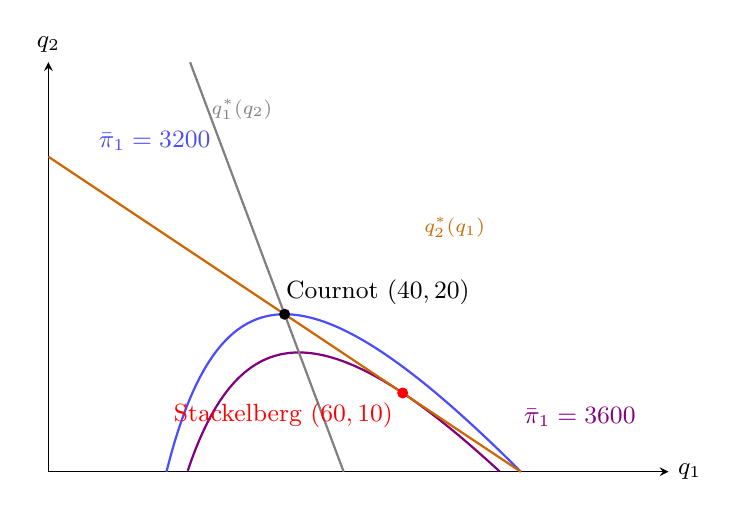
\begin{tikzpicture}[x=0.075cm,y=0.1cm,font=\small,>=stealth]
  \draw[->] (0,0) -- (105,0) node[right] {$q_1$};
  \draw[->] (0,0) -- (0,52) node[above] {$q_2$};
  \draw[thick,blue!70,domain=20:80,samples=80,smooth] plot (\x,{100-\x-1600/\x});
  \draw[thick,violet,domain=23.6:76.4,samples=80,smooth] plot (\x,{100-\x-1800/\x});
  \draw[thick,gray] (24,52) -- (50,0);
  \draw[thick,orange!80!black] (0,40) -- (80,0);
  \fill (40,20) circle (2pt) node[above right,xshift=-3pt] {Cournot $(40,20)$};
  \fill[red] (60,10) circle (2pt) node[below left,red] {Stackelberg $(60,10)$};
  \node[blue!70] at (18,42) {$\bar\pi_1=3200$};
  \node[violet] at (90,7) {$\bar\pi_1=3600$};
  \node[orange!80!black,font=\scriptsize,anchor=west] at (62,31) {$q_2^*(q_1)$};
  \node[gray,font=\scriptsize,anchor=west] at (26,46) {$q_1^*(q_2)$};
\end{tikzpicture}
\end{center}
(La recta decreciente naranja es la función de reacción de la firma 2, $q_2 = 40 - \frac{q_1}{2}$; la recta gris, $q_2 = 100 - 2q_1$, es la función de reacción de la firma 1, $q_1 = 50 - \frac{q_2}{2}$.)

\end{solution}

\part Suponga que las dos empresas de la industria se comportan à la Stackelberg (en cantidad), de modo que la empresa 1 actúa como líder y la 2 como seguidora. ¿Cuál sería la producción y el precio de equilibrio de mercado? ¿Cuánto producirá la empresa 1? ¿Y la empresa 2? ¿Cuáles serán los beneficios de ambas empresas?
\needspace{5\baselineskip}
\begin{solution}
Se resuelve por inducción hacia atrás (ver el ejercicio anterior de Stackelberg con estos mismos datos): $q_1^* = 60$, $q_2^* = 10$, $Q^* = 70$, $P^* = 100$, $\pi_1 = 3600$ y $\pi_2 = 200$.

\end{solution}
\end{parts}

%-------------------------------------------------------------------- Stackelberg con inversión
\needspace{8\baselineskip}
\tema{Stackelberg con inversión para convertirse en líder}
\question Considere una industria con dos empresas, $L$ y $S$, que producen un producto homogéneo. La empresa $L$ es la líder y la $S$ la seguidora. La función inversa de demanda es $p(q_L,q_S) = 1 - q_L - q_S$, donde $q_L$ y $q_S$ son las cantidades producidas por la líder y la seguidora, respectivamente, y $p$ es el precio de mercado. Suponga además que la función de costos es $C_i(q_i) = \frac{1}{2}q_i$, para $i = L,S$.
\begin{parts}
\part Calcule las producciones en equilibrio, el precio de mercado, las cuotas de mercado y el beneficio de cada empresa.
\needspace{5\baselineskip}
\begin{solution}
Por inducción hacia atrás, la seguidora resuelve $\max_{q_S}\ (\frac{1}{2} - q_L - q_S)q_S$, de donde $q_S(q_L) = \frac{1}{4} - \frac{q_L}{2}$. La líder resuelve
\[
  \max_{q_L}\ \Bigl(\tfrac{1}{2} - q_L - \tfrac{1}{4} + \tfrac{q_L}{2}\Bigr)q_L = \Bigl(\tfrac{1}{4} - \tfrac{q_L}{2}\Bigr)q_L
  \;\Rightarrow\; q_L^* = \frac{1}{4}, \qquad q_S^* = \frac{1}{8}.
\]
Así, $Q = \frac{3}{8}$ y $p = \frac{5}{8}$. Las cuotas de mercado son $\frac{2}{3}$ para $L$ y $\frac{1}{3}$ para $S$, y los beneficios son $\pi_L = \frac{1}{8}\cdot\frac{1}{4} = \frac{1}{32}$ y $\pi_S = \frac{1}{8}\cdot\frac{1}{8} = \frac{1}{64}$.

\end{solution}

\part Suponga que las empresas compiten en cantidades simultáneamente (Cournot). Calcule las cantidades de equilibrio, el precio, las cuotas y los beneficios, y compare su respuesta con la anterior.
\needspace{5\baselineskip}
\begin{solution}
Cada firma resuelve $\max_{q_i}\ (\frac{1}{2} - q_i - q_j)q_i$, de modo que $q_i = \frac{1/2 - q_j}{2}$ y $q_L^* = q_S^* = \frac{1}{6}$. Entonces $Q = \frac{1}{3}$, $p = \frac{2}{3}$, las cuotas son $\frac{1}{2}$ cada una y $\pi_L = \pi_S = \frac{1}{6}\cdot\frac{1}{6} = \frac{1}{36}$.

Comparando con Stackelberg: la cantidad total es mayor y el precio menor ($\frac{5}{8} < \frac{2}{3}$); la líder gana más ($\frac{1}{32} > \frac{1}{36}$) y la seguidora gana menos ($\frac{1}{64} < \frac{1}{36}$) que en Cournot.

\end{solution}

\part Suponga que las empresas compiten en cantidades secuencialmente, pero ahora la empresa $S$ puede invertir $\bar S$ y convertirse en líder. ¿Debería la seguidora invertir? ¿Cómo depende su decisión del valor de $\bar S$?
\needspace{5\baselineskip}
\begin{solution}
Si $S$ invierte, se convierte en líder y obtiene el beneficio de la líder menos la inversión, $\frac{1}{32} - \bar S$. Si no invierte, queda como seguidora y obtiene $\frac{1}{64}$. Por lo tanto, $S$ debe invertir si y solo si
\[
  \frac{1}{32} - \bar S > \frac{1}{64}
  \quad\Longleftrightarrow\quad
  \bar S < \frac{1}{64}.
\]
Es decir, la seguidora invierte solo si el costo de la inversión es menor que la ganancia de ser líder en lugar de seguidora.

\end{solution}
\end{parts}

%-------------------------------------------------------------------- Juego de inversión del monopolista
\needspace{8\baselineskip}
\tema{Juego secuencial: inversión del monopolista y entrada}
\question Considere un juego secuencial donde un monopolista puede invertir en tecnología antes de la potencial entrada de un competidor. Si el monopolista invierte, la estructura de pagos favorece la estrategia de guerra en caso de entrada del competidor. El monopolista elige primero entre invertir ($I$) o no invertir ($NI$). Luego el competidor debe decidir entre entrar ($E$) o no entrar ($NE$) al mercado, y si entra el monopolista elige entre acomodar ($A$) o iniciar una guerra de precios ($G$). Los pagos (monopolista, entrante) son:
\begin{center}
\renewcommand{\arraystretch}{1.1}
\begin{tabular}{llc}
  Invierte & Entra y guerra ($I,E,G$) & $(10,-10)$ \\
  Invierte & Entra y acomoda ($I,E,A$) & $(0,20)$ \\
  Invierte & No entra ($I,NE$) & $(30,0)$ \\
  No invierte & No entra ($NI,NE$) & $(50,0)$ \\
  No invierte & Entra y guerra ($NI,E,G$) & $(-10,-10)$ \\
  No invierte & Entra y acomoda ($NI,E,A$) & $(20,20)$
\end{tabular}
\end{center}
\begin{parts}
\part Obtenga el equilibrio perfecto en subgrupos (subjuegos) del anterior juego secuencial.
\needspace{5\baselineskip}
\begin{solution}
Resolvemos desde abajo hacia arriba. El último en elegir es el monopolista, que decide entre guerra ($G$) o acomodar ($A$) en el caso de que el competidor decida entrar. En el lado izquierdo, cuando el monopolista invirtió, optará por una guerra de precios, pues obtiene mayores beneficios ($10 > 0$). De la misma forma, en el lado derecho, cuando el monopolista no invierte, preferirá acomodar al competidor ($20 > -10$).

Luego, el competidor decide entre entrar ($E$) o no entrar ($NE$), sabiendo lo que hará el monopolista. Si el monopolista invirtió, el competidor decidirá no entrar ($0 > -10$). Si el monopolista decidió no invertir, el competidor elegirá entrar ($20 > 0$).

Finalmente, el monopolista, sabiendo todo lo anterior, sabe que si invierte tendrá un pago de $30$, mientras que al no invertir tendrá un pago de $20$; por lo tanto, decide realizar la inversión, ya que esta (en el sentido económico) amenaza al entrante, persuadiéndolo de no entrar, aunque con un costo asociado: hubiera obtenido un mejor pago ($50$) si no hubiera invertido y el competidor no entrara. El equilibrio perfecto en subjuegos es $\{(I,G,A),\ (NE,E)\}$, con pagos $(30,0)$.

\end{solution}

\part Escriba el juego secuencial en su forma normal.
\needspace{5\baselineskip}
\begin{solution}
Las estrategias del monopolista son (decisión de invertir, acción si hay entrada tras $I$, acción si hay entrada tras $NI$); las del entrante son (acción tras $I$, acción tras $NI$):
\begin{center}
\renewcommand{\arraystretch}{1.1}
\begin{tabular}{l|cccc}
  & $E,NE$ & $E,E$ & $NE,NE$ & $NE,E$ \\ \hline
  $I,G,G$ & $10,-10$ & $10,-10$ & $30,0$ & $30,0$ \\
  $I,G,A$ & $10,-10$ & $10,-10$ & $30,0$ & $30,0$ \\
  $I,A,G$ & $0,20$ & $0,20$ & $30,0$ & $30,0$ \\
  $I,A,A$ & $0,20$ & $0,20$ & $30,0$ & $30,0$ \\
  $NI,G,G$ & $50,0$ & $-10,-10$ & $50,0$ & $-10,-10$ \\
  $NI,G,A$ & $50,0$ & $20,20$ & $50,0$ & $20,20$ \\
  $NI,A,G$ & $50,0$ & $-10,-10$ & $50,0$ & $-10,-10$ \\
  $NI,A,A$ & $50,0$ & $20,20$ & $50,0$ & $20,20$
\end{tabular}
\end{center}

\end{solution}

\part Encuentre un equilibrio de Nash en forma normal que lleve a un resultado diferente al de la solución en (a).
\needspace{5\baselineskip}
\begin{solution}
En este juego simultáneo aparecen distintos equilibrios de Nash, como el par de estrategias $(NI,G,G)$ y $(E,NE)$, con pagos $(50,0)$: el monopolista no invierte y amenaza con guerra si hay entrada, y el entrante no entra tras $NI$ porque anticipa la guerra (el monopolista no tiene incentivos a cambiar, pues obtiene el máximo $50$, y el entrante tampoco). Esto se debe a que en la forma normal las decisiones se toman al mismo tiempo y se pierde la información secuencial crucial del juego: la amenaza de guerra tras $NI$ no es creíble en el juego secuencial (acomodar da $20 > -10$), pero resulta ser un equilibrio de Nash válido en la forma normal. Esto ilustra por qué fue desarrollado el concepto de equilibrio perfecto en subjuegos: para eliminar equilibrios basados en amenazas no creíbles que, aunque matemáticamente consistentes en la forma normal, no reflejan el comportamiento racional esperado cuando las decisiones se toman secuencialmente.

\end{solution}
\end{parts}

%-------------------------------------------------------------------- Stackelberg con costo fijo
\needspace{8\baselineskip}
\tema{Cournot y Stackelberg con costos asimétricos y costo fijo (líder 1 o 2)}
\question Asuma que existen 2 firmas que producen un bien homogéneo. Sus funciones de costos vienen dadas por $C_1(q_1) = 20q_1 + 1$ y $C_2(q_2) = 30q_2$. La curva de demanda inversa en el mercado es $P = 60 - 5Q$.
\begin{parts}
\part Si ambas firmas compiten à la Cournot, ¿cuál es el precio de equilibrio? ¿Cuál es el nivel de producción y beneficios de cada firma?
\needspace{5\baselineskip}
\begin{solution}
Firma 1: $\max_{q_1}\ (60 - 5q_1 - 5q_2 - 20)q_1 - 1$, con CPO $40 - 10q_1 - 5q_2 = 0$, es decir, $q_1 = 4 - \frac{q_2}{2}$. Firma 2: $\max_{q_2}\ (60 - 5q_1 - 5q_2 - 30)q_2$, con CPO $30 - 5q_1 - 10q_2 = 0$, es decir, $q_2 = 3 - \frac{q_1}{2}$. Reemplazando: $q_1 = 4 - \frac{3 - q_1/2}{2}$, de donde $\frac{3}{4}q_1 = \frac{5}{2}$ y
\[
  q_1^C = \frac{10}{3}, \qquad q_2^C = \frac{4}{3}, \qquad Q = \frac{14}{3}, \qquad P^C = 60 - 5\cdot\frac{14}{3} = \frac{110}{3},
\]
\[
  \pi_1^C = \Bigl(\frac{110}{3} - 20\Bigr)\frac{10}{3} - 1 = \frac{491}{9} \approx 54{,}56, \qquad
  \pi_2^C = \Bigl(\frac{110}{3} - 30\Bigr)\frac{4}{3} = \frac{80}{9} \approx 8{,}89 .
\]

\end{solution}

\part Suponga que ambas firmas se comportan à la Stackelberg (en cantidad), de modo que la empresa 1 actúa como líder y la 2 como seguidora. ¿Cuánto producirán las firmas 1 y 2? Calcule el nuevo precio de equilibrio y los beneficios de cada firma.
\needspace{5\baselineskip}
\begin{solution}
Por inducción hacia atrás, en $t=2$ la seguidora tiene $q_2(q_1) = 3 - \frac{q_1}{2}$. La líder maximiza
\[
\begin{gathered}
  \max_{q_1}\ \Bigl(60 - 5q_1 - 5\bigl(3 - \tfrac{q_1}{2}\bigr) - 20\Bigr)q_1 - 1 = (25 - 2{,}5q_1)q_1 - 1 \\
  \Longrightarrow\; 25 - 5q_1 = 0 \;\Longrightarrow\; q_1 = 5 .
\end{gathered}
\]
Por lo tanto $q_2 = 3 - \frac{5}{2} = \frac{1}{2}$, $Q = \frac{11}{2}$ y $P = 60 - 5\cdot\frac{11}{2} = 32{,}5$. Los beneficios son
\[
  \pi_1 = (32{,}5 - 20)\cdot 5 - 1 = 61{,}5, \qquad \pi_2 = (32{,}5 - 30)\cdot\frac{1}{2} = 1{,}25 .
\]

\end{solution}

\part ¿Cómo cambia su respuesta en (b) si la firma 2 es la líder?
\needspace{5\baselineskip}
\begin{solution}
Ahora la firma 1 es seguidora, con $q_1(q_2) = 4 - \frac{q_2}{2}$. La líder 2 maximiza
\[
  \max_{q_2}\ \Bigl(60 - 5\bigl(4 - \tfrac{q_2}{2}\bigr) - 5q_2 - 30\Bigr)q_2 = (10 - 2{,}5q_2)q_2
  \;\Longrightarrow\; q_2 = 2 .
\]
Entonces $q_1 = 3$, $Q = 5$ y $P = 60 - 25 = 35$. Los beneficios son $\pi_1 = (35 - 20)\cdot 3 - 1 = 44$ (seguidora) y $\pi_2 = (35 - 30)\cdot 2 = 10$ (líder). Dada la asimetría de costos, cuando la firma 2 (de mayor costo) actúa como líder se observa una menor oferta en el mercado y un precio más alto; la firma 2 produce menos y obtiene menores beneficios en comparación con la firma 1, pero estos beneficios son superiores a los que obtenía cuando actuaba como seguidora.

\end{solution}

\part ¿Qué tipo de competencia le conviene a las firmas 1 y 2?
\needspace{5\baselineskip}
\begin{solution}
Comparamos los beneficios en cada caso. Para la firma 1: $\pi_1^{\text{líder}} = 61{,}5 > \pi_1^{C} = 54{,}56 > \pi_1^{\text{seguidora}} = 44$. Para la firma 2: $\pi_2^{\text{líder}} = 10 > \pi_2^{C} = 8{,}89 > \pi_2^{\text{seguidora}} = 1{,}25$. Por lo tanto, a ambas firmas les conviene competir à la Stackelberg actuando como líderes; si actúan como seguidoras, les resulta más beneficioso competir à la Cournot.

\end{solution}
\end{parts}
